%% V1.0
%% by Gabriel Garcia, gabrcg@gmail.com
%% This is a template for Udacity projects using IEEEtran.cls

%% Be Udacious!

\documentclass[10pt,journal,compsoc]{IEEEtran}

\usepackage[pdftex]{graphicx}
\usepackage{cite}
\usepackage{booktabs}
\usepackage{listings}
\lstset{basicstyle=\ttfamily,
  breaklines=true}
\usepackage{hyperref}
\hypersetup{
    colorlinks=true,
    linkcolor=blue,
    filecolor=magenta,
    urlcolor=cyan,
}
\usepackage{comment}
\hyphenation{op-tical net-works semi-conduc-tor}


\begin{document}

\title{RoboND: Robot Localization Project}

\author{Matthew Dewar}

\markboth{Localization project, Robotics Nanodegree Program, Udacity, Monte Carlo Localization, Kalman Filter}%
{}
\IEEEtitleabstractindextext{%

\begin{abstract}
In this project two mobile robot models are created and evaluated within a maze environment to be able to navigate to a predefined goal position. Both robots contain a camera and a laser scanner to process its environment for use in the navigation stack. Adaptive Monte Carlo Localization (AMCL) is used on both robots to localize within the global environment. Parameters of both the AMCL, and the Move-Base packages are tuned to optimize navigation performance.
\end{abstract}

% Note that keywords are not normally used for peer review papers.
\begin{IEEEkeywords}
Robot, IEEEtran, Udacity, \LaTeX, Localization.
\end{IEEEkeywords}}


\maketitle
\IEEEdisplaynontitleabstractindextext
\IEEEpeerreviewmaketitle
\section{Introduction}
\label{sec:introduction}

\IEEEPARstart{A}{} critical ability for a mobile robot is for it to be able to locate itself within an environment, asking the question "Where am I?". While localization may be fairly trivial in a perfect environment with perfect sensors, in the real world noisy sensors with large uncertainties, and compounding errors from odometry data drastically complicate the problem. Moreover, multiple sensors will most likely need to be used and compounded in order to achieve an accurate enough sensor measurement, labeled as sensor fusion.

The three most common problems in localization are position tracking, global localization, and the kidnapped robot problem. Position tracking involves the robot knowings its initial position, and then estimating its pose as it moves around the environment \cite{UdacityLesson9}. With global localization the robot's initial pose is unknown and it must determine its position relative to the ground truth map. The global localization problem is harder than the position tracking problem. Lastly, the kidnapped robot problem is the same as the global localization problem, however the robot may be kidnapped at any time, and replaced within the environment.

For this project the global localization project will be addressed creating a program using the Robot operating System \cite{ROSWiki}, along with the Adaptive Monte Carlo Localization (AMCL) package for localizing, \cite{ROSAMCL}, and the move\_base package for interacting with the navigation stack on the robot \cite{ROSMoveBase}. This program will be able to globally localize two different robots within a supplied environment (Figure. \ref{fig:environment}), and navigate the robot to the goal position determined by Udacity.

\begin{figure}[thpb]
      \centering
      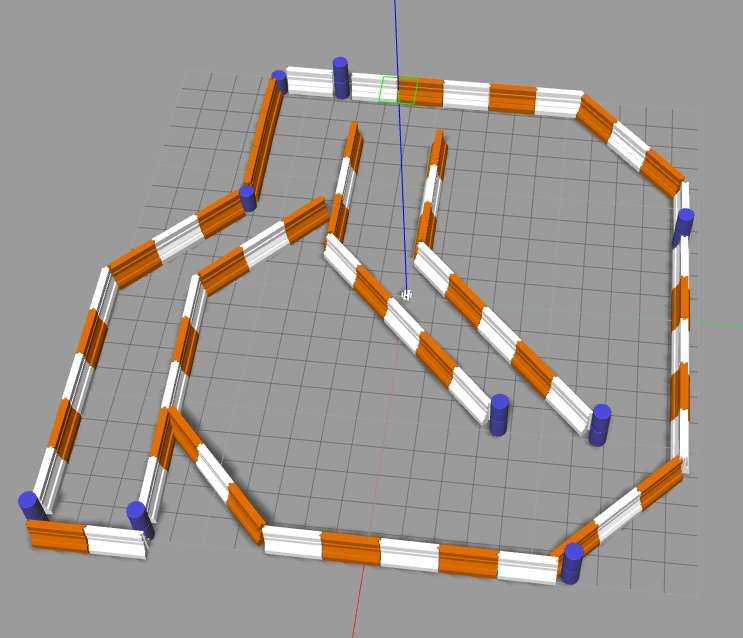
\includegraphics[width=\linewidth]{../img/map-overview.png}
      \caption{Environment for testing the navigation and localization stack for both the benchmark and custom robots.}
      \label{fig:environment}
\end{figure}

\section{Background}

The typical navigation stack for a mobile robot consists of odometery and sensor data used in conjunction with a ground truth map, which is then fed into the move\_base node which outputs motion commands to the base controller to move the robot (see Figure. \ref{fig:navstack}). Inside the move\_base node, local and global costmaps are developed and divided into unoccupied regions, walls, and obstacles. An optional localization node can then be added into the navigation stack to locate the robot within the ground truth map. Porting this stack over to a real world robot, localization will also help with the noisy and uncertain data the robot will obtain. The two most used algorithms for localization are the Extended Kalman filter (EKF), and the Adaptive Monte Carlo Localization (AMCL).

%example for inserting image
\begin{figure}[thpb]
      \centering
      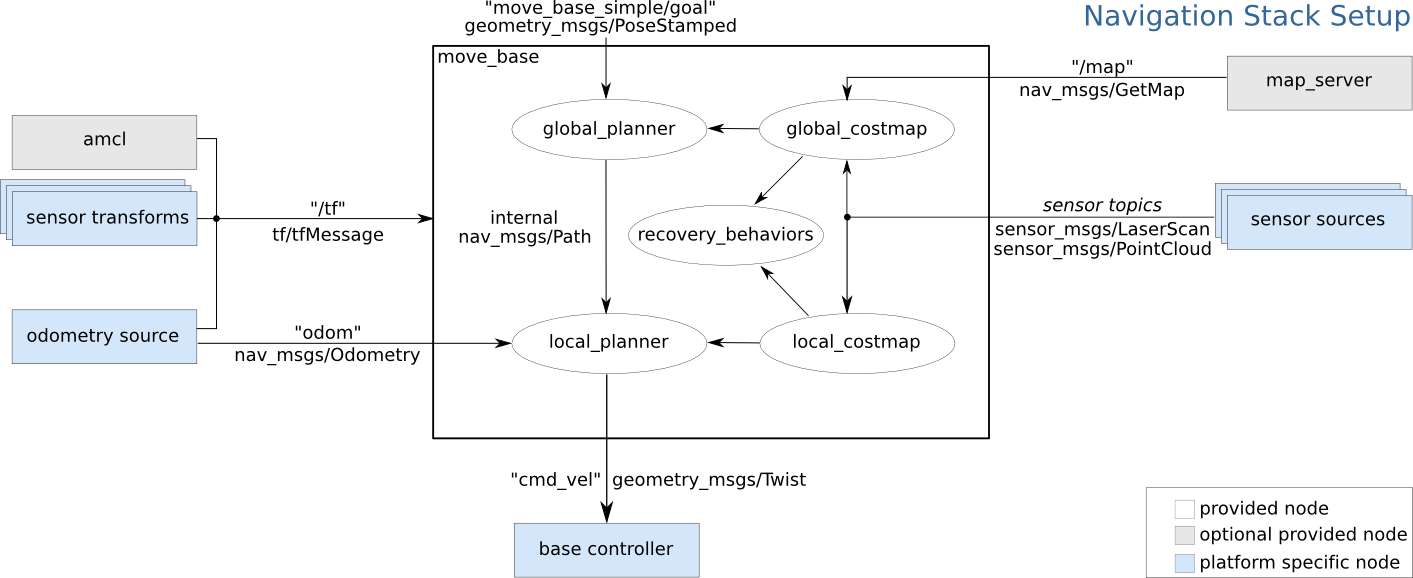
\includegraphics[width=\linewidth]{../img/overview_tf.png}
      \caption{Navigation stack for the robot, using odometry and sensor data along with AMCL into the move-base node where the robot sensors and the ground truth map are used to create a global and local costmap where velocity, and orientation commands are then sent to the base controller for motion.}
      \label{fig:navstack}
\end{figure}

\subsection{Kalman Filters}
The Kalman filter is an algorithm commonly used in guidance, navigation, and control systems for filtering out statistical noise and other inaccuracies from measurement data, producing an estimate of the systems state \cite{kalmanwiki}. This state estimate is obtained by providing an initial estimate, whereby sensors measurements can gain knowledge about our environment increasing confidence in the system's state (Figure \ref{fig:posteriorState}), where control actions cause some change in the system's state and a new state prediction is made. In robotics this filtering approach can be used to predict the current location of the robot with appropriate data allocated from multiple range finding sensors (i.e. lidars, and depth cameras). However, the traditional Kalman filter is limited to linear motions and measurement functions, whereby the Extended Kalman Fitler (EKF) is employed to linearize the nonlinear functions approximated via Taylor series \cite{UdacityLesson10}. To adapt the EKF to multidimensional cases, Jacobians are employed to linearized the measurement and state covariances.

\begin{figure}[thpb]
      \centering
      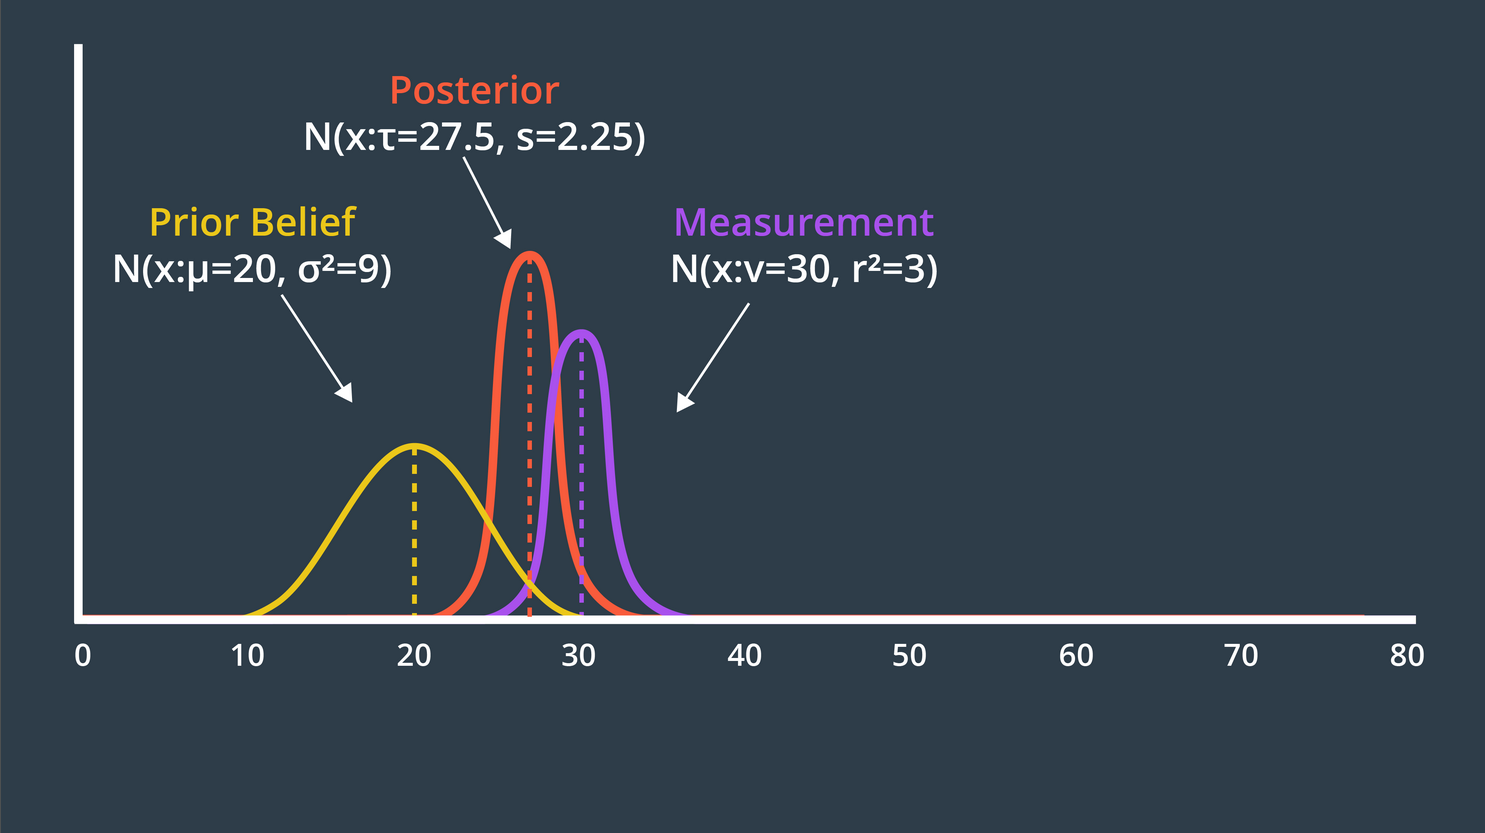
\includegraphics[width=\linewidth]{../img/Bayes_Theorem.png}
      \caption{A prior belief of a robots location can be improved by providing a measurement update to the prior belief of the system, where a more confident posterior belief can result.}
      \label{fig:posteriorState}
\end{figure}


\subsection{Particle Filters}

In Monte Carlo Localization the robots position and orientation are represented by a set a particles distributed around the map predicting the state of the robot. The initial pose of the robot can be known or unknown, where a recursive Bayes filter can measure the posterior state through a prediction step, and then a measurement update step. In the prediction step, motion commands are given to the particles and updated on the map. Then in the measurement update step, sensor measurements to mapped landmarks are compared to each particles position. Each particle is then given a weighted probability that it could be the robots current location, and the particles are then redistributed in the next time step based on this probability \cite{PEEL2018244}. The accumulated probability mass of the particles is used as the current pose of the robot at that time step. In Adaptive Monte-Carlo Localization (AMCL) "the number of particles are adapted over time using Kullback-Leibler Divergence Sampling (KLD-Sampling) to determine the number of particles that are required at each time step" \cite{PEEL2018244}. After many time steps the posterior state of the particles should become more confident and cluster around a single location, given an accurate estimate of the current robot's pose, Figure \ref{fig:AMCL_particles}.

\begin{figure}[thpb]
    \centering
    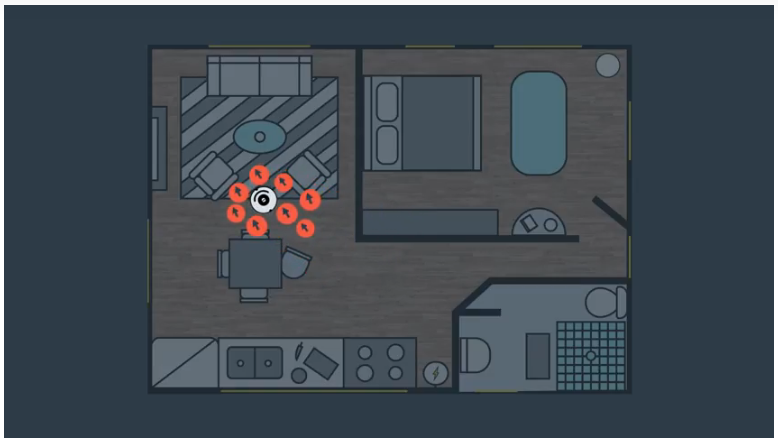
\includegraphics[width=\linewidth]{../img/amcl_particles.png}
    \caption{Illustration of AMCL after multiple time steps where the particles are seen to converge and mass upon a single location on the map.}
    \label{fig:AMCL_particles}
\end{figure}

\subsection{Comparison / Contrast}
The AMCL can be seen to have many advantages over the Extended Kalman Filter, illustrated in Figure \ref{fig:FilterComparision}. The EKF is limited to a linear Gaussian state space, where the AMCL is not. The AMCL is easier to implement, and the computational memory and resolution of the AMCL can be controlled by tuning parameters related to particle quantity and distribution. The EKF on the other hand is useful for systems that require higher resolutions, and limited in computational power. In this paper AMCL will be chosen as the localization algorithm due to its ability to handle non-linear states.

\begin{figure}[thpb]
    \centering
    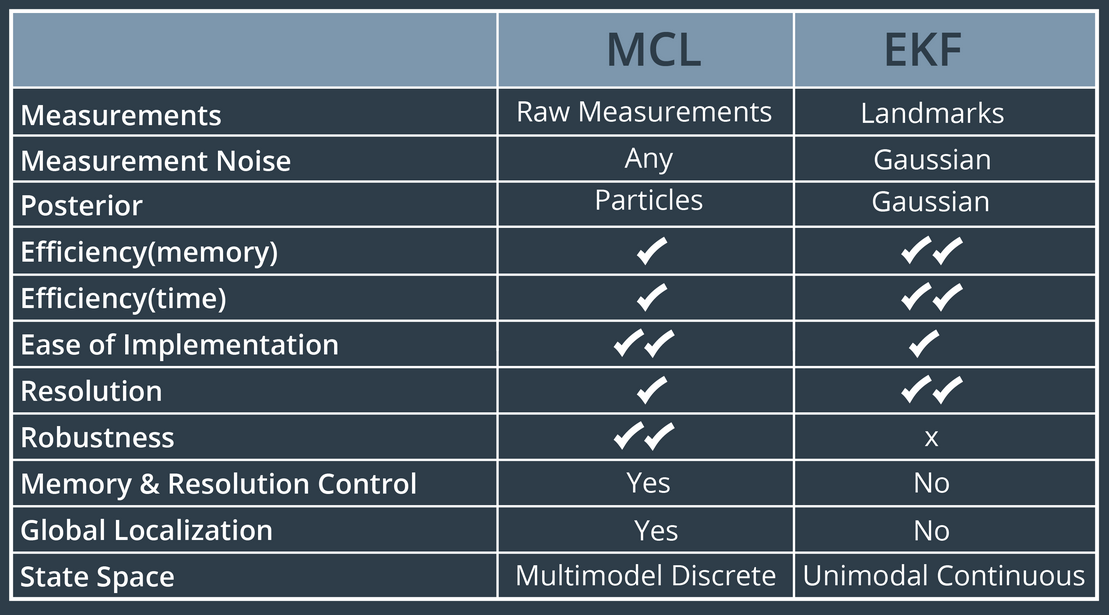
\includegraphics[width=\linewidth]{../img/mclvsekf.png}
    \caption{}
    \label{fig:FilterComparision}
\end{figure}

\section{Simulations}
Within ROS, Gazebo was chosen to simulate the environment which the robot will navigate. A Premade environment located in \textit{$/maps/jackal\_race.world$} will be used to test the robot's navigation abilities. RViz was then used to visualize both the robot, and the sensor measurements, as well as to view the particle pose array created with the AMCL package, and the cost maps developed with the Move\_Base package. The proper RViz configuration, and gazebo environment will load by issuing the command:

\begin{lstlisting}
    roslaunch udacity_bot udacity_world.launch
\end{lstlisting}

For the robot supplied by Udacity, and:

\begin{lstlisting}
    roslaunch tank_bot tank_world.launch
\end{lstlisting}

For the custom robot made by the author.


Tuning parameters for the local planner, and cost maps used in the navigation stack can be found in the \textit{$/config/$} folder for both the udacity\_bot, and tank\_bot repositories. They are broken up into four files:

\begin{itemize}

    \item local\_costmap\_params.yaml
    \item global\_costmap\_params.yaml
    \item costmap\_common\_params.yaml
    \item base\_local\_planner\_params.yaml

\end{itemize}

Tuning of the parameters located in these files will be discussed below and in subsequent sections.

URDF files for the baseline robot model and the custom model are found in the \textit{$/urdf/$} file for each robot, where they are broken up into a \textit{$/.xacro/$}, and a \textit{$/.gazebo/$} file in order to define simulation parameters for the drive controller, camera, and laser range finder.

\begin{comment}
This section should discuss the performance of robots in simulation. Items to include are the robot model design, packages used, and the parameters chosen for the robot to properly localize itself. The information provided here is critical if anyone would like to replicate your results. After all, the intent of reports such as these are to convey information and build upon ideas so you want to ensure others can validate your process.
You should have at least two images here: one that shows your standard robot used in the first part of the project, and a second robot that you modified / built that is different from the first robot. Remember to watermark all of your images as well.
\end{comment}

\subsection{Achievements}
The baseline robot successfully completed moving to the navigation goal in 1 minute and 47 seconds. Multiple runs of the navigation goal script were tested, and were all successful. 2D nav goals around the map were tested, with the baseline robot successfully moving around the environment.

% Robot Models
\subsection{Benchmark Model}
\subsubsection{Model design}

The Udacity-bot seen in Figure. \ref{fig:udacity-bot-design} consists of a 0.4m X 0.2m X 0.1m rectangular body with two 0.1m radius wheels on either side, and front and back caster balls for stability. Sensors on the robot consist of a front facing camera on the front of the robot's body, and a Hokuyo Scanning Laser Rangefinder on top of the robot. The full description of the robot can be found in \textit{$udacity\_bot/urdf/udacity\_bot.xacro$}, and \textit{$udacity\_bot/urdf/udacity\_bot.gazebo$}.

\begin{figure}[thpb]
    \centering
    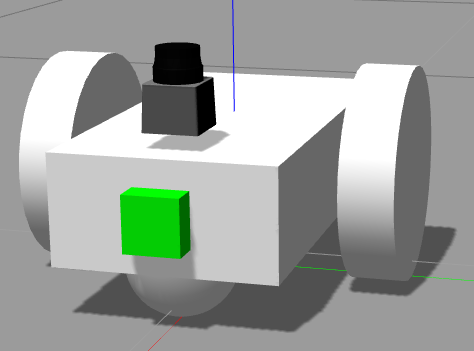
\includegraphics[width=\linewidth]{../img/urdf_udacity_bot.png}
    \caption{Udacity\_bot rendered in Gazebo.}
    \label{fig:udacity-bot-design}
\end{figure}

\subsubsection{Parameters}

Optimal parameters for the benchmark model can be divided into relevant parameters for the AMCL node, Table. \ref{tab:AMCLparam-Udacitybot}, and for the costmaps nodes of the move-base navigation package, Table. \ref{tab:costmapParam-Udacitybot}. Minimizing the number of particle in the adaptive AMCL helped increase the certainty and the performance of the AMCL only after a few time steps. Transform tolerances defining the latency between transforms in both the AMCL, and costmap node were set just high enough to avoid a transform timeout error. The inflation radius was set appropriately for the robot to be able to navigate within tight spaces, but not run into any obstacles. Relatively high values for the obstacle range and inflation range were used to give the robot a high enough field of view to be able to make the best navigation planner. Update and publish frequencies are mainly dependant on system performance and how quickly the costmaps can be updated. For this report, validation and testing was performed on a local machine with a Intel Core i5 CPU at 3.2GHz with 8GB of RAM. A full list of parameters can be found in the \textit{$udacity\_bot/config/$} directory.

\begin{table}[ht]
\caption{AMCL parameters for the benchmark model.}
\label{tab:AMCLparam-Udacitybot}
\begin{center}
    \begin{tabular}{ll}
        \toprule%
    \multicolumn{2}{l}{\textbf{AMCL Node Parameters}} \\
    \midrule
    min particles              & 50                   \\
    max particles              & 200                  \\
    KLD error                  & 0.1                  \\
    KLD-Z                      & 0.99                 \\
    transform\_tolerance       & 0.2                  \\
    recovery\_alpha\_slow      & 0.001                \\
    recovery\_alpha\_fast      & 0.1                  \\
    \midrule
    \multicolumn{2}{l}{\textbf{AMCL Laser}}           \\
    \midrule
    laser\_min\_range          & 0.1                  \\
    laser\_max\_range          & 30.0                 \\
    laser\_max\_beams          & 50                   \\
    laser model type           & likelihood field     \\
    \midrule
    \multicolumn{2}{l}{\textbf{AMCL Odometery}}       \\
    \midrule
    odom\_model\_type          & diff                 \\
    odom\_alpha                & 0.2                   \\
    \bottomrule
    \end{tabular}
\end{center}
\end{table}

\begin{table}[ht]
\caption{AMCL parameters for the benchmark model.}
\label{tab:costmapParam-Udacitybot}
\begin{center}
    \begin{tabular}{lcc}
        \toprule%
\textbf{Parameters} & \textbf{Global}  & \textbf{Local}   \\
\midrule
global frame        & map              & odom             \\
robot base frame    & robot\_footprint & robot\_footprint \\
update frequency    & 10               & 10               \\
publish frequency   & 10               & 10               \\
width               & 5                & 5                \\
height              & 5                & 5                \\
resolution          & 0.07             & 0.05             \\
obstacle range      & 3                & 3                \\
raytrace range      & 5                & 5                \\
transform tolerance & 0.5              & 0.5              \\
robot radius        & 0.5              & 0.5              \\
inflation radius    & 0.6              & 0.6             \\
    \bottomrule%
\end{tabular}
\end{center}
\end{table}



\begin{comment}
Localization parameters in the AMCL node should be described, as well as move\_base parameters in the configuration file. You should be able to clearly demonstrate your understanding of the impact of these parameters.
\end{comment}

\subsection{Personal Model}
% ditto
\subsubsection{Model design}

The personal robot designed for this project, named Tank-bot, was made to provide a platform where this software package could be adapted for outdoor environments where a variable landscape, and objects that the robot could travel over are handled. Tank-bot consists of three wheels on each side with a rounded-bottom body to be able to roll over minor obstacles. Initially the front and back wheels were set higher up the body than the middle wheels to be able to adapt to variable terrain; however, for the environment in Figure. \ref{fig:environment} the robot was not able to navigate appropriately. Therefore all of the wheels were set to same height with the differential drive set to the rear wheels. The robot model was created in Blender, where the collision, inertial, and joint objects were created with a robot model creation plug-in called Phobos \cite{phobos}. The Phobos environment for creating URDF files can be seen in Figure. \ref{fig:phobos-env}. A camera, and laser scanner were used for robot sensors similar to the benchmark robot with the camera in the front, and the laser scanner on top. Figure. \ref{fig:tank-bot-design} shows the Tank-bot rendered in blender.

\begin{figure}[thpb]
    \centering
    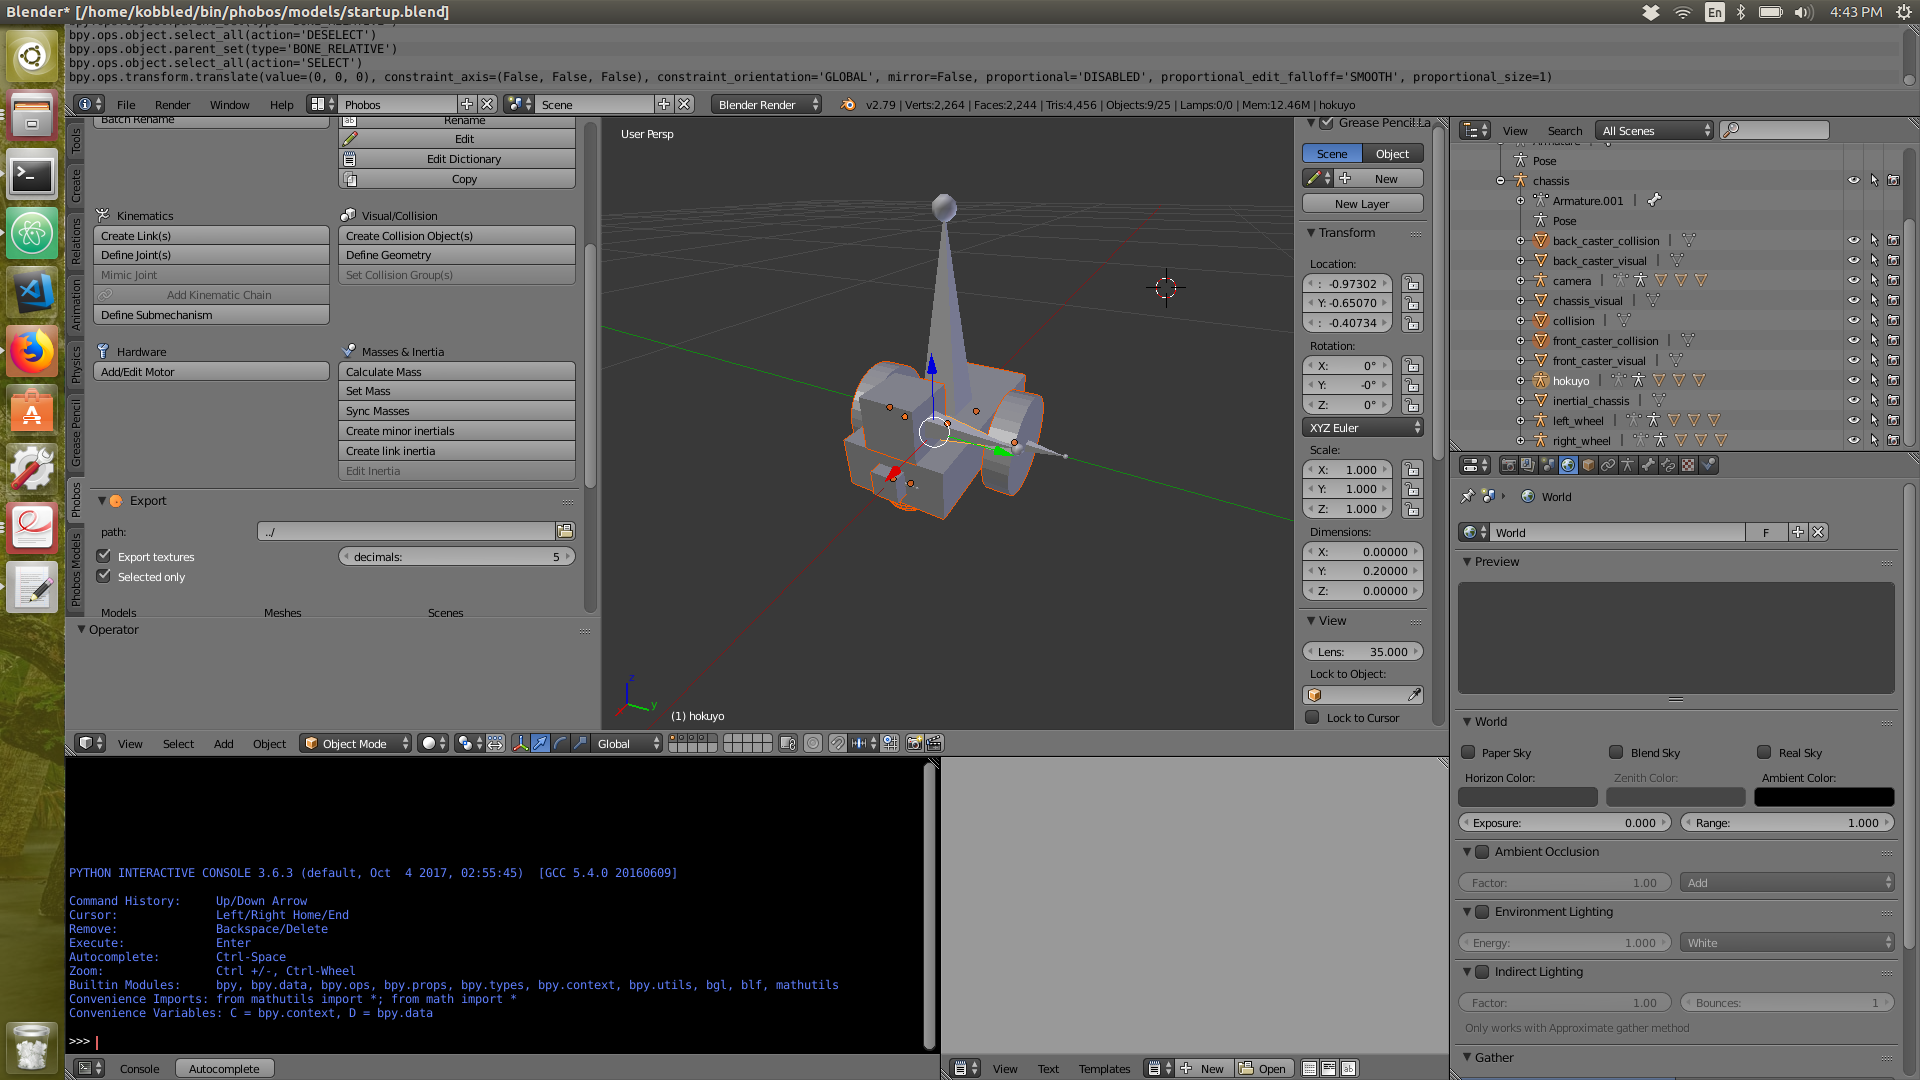
\includegraphics[width=\linewidth]{../img/phobos_env.png}
    \caption{The Phobos add-on environment for blender used to export URDF files for use as a robot model.}
    \label{fig:phobos-env}
\end{figure}

\begin{figure}[thpb]
    \centering
    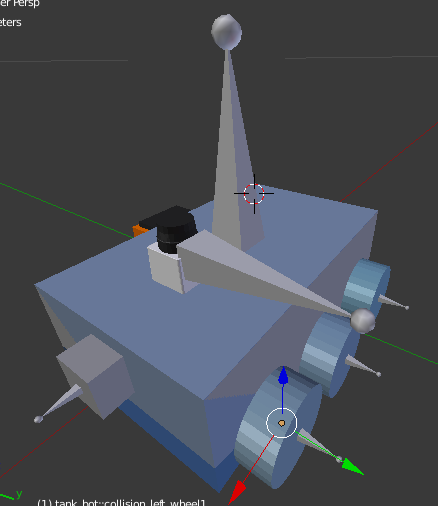
\includegraphics[width=\linewidth]{../img/urdf_tank_bot.png}
    \caption{Tank\_bot rendered in Blender using the Phobos add-on to visualize the URDF file.}
    \label{fig:tank-bot-design}
\end{figure}

\subsubsection{Parameters}

AMCL parameters in \ref{tab:AMCLparam-Tankbot}, and costmap parameters in \ref{tab:costmapParam-Tankbot} for the Tank-bot had to be modified compared to the benchmark model in order for the robot to be able to move within the environment. Without the modifications in the parameters provided, the robot was unable to navigate during any 2D nav goal operations. Even with these modification the tank-bot has difficulty localizing and navigation in its environment from its initial pose. A full list of parameters can be found in the \textit{$tank\_bot/config/$} directory.

\begin{table}[ht]
\caption{AMCL parameters for the personal model.}
\label{tab:AMCLparam-Tankbot}
\begin{center}
    \begin{tabular}{ll}
        \toprule%
    \multicolumn{2}{l}{\textbf{AMCL Node Parameters}} \\
    \midrule
    min particles              & 25                   \\
    max particles              & 200                  \\
    KLD error                  & 0.05                  \\
    KLD-Z                      & 0.99                 \\
    transform\_tolerance       & 0.2                  \\
    recovery\_alpha\_slow      & 0.001                \\
    recovery\_alpha\_fast      & 0.1                  \\
    \midrule
    \multicolumn{2}{l}{\textbf{AMCL Laser}}           \\
    \midrule
    laser\_min\_range          & 0.1                  \\
    laser\_max\_range          & 30.0                 \\
    laser\_max\_beams          & 50                   \\
    laser model type           & likelihood field     \\
    \midrule
    \multicolumn{2}{l}{\textbf{AMCL Odometery}}       \\
    \midrule
    odom\_model\_type          & diff                 \\
    odom\_alpha                & 0.2                   \\
    \bottomrule
    \end{tabular}
\end{center}
\end{table}

\begin{table}[ht]
\caption{AMCL parameters for the personal model.}
\label{tab:costmapParam-Tankbot}
\begin{center}
    \begin{tabular}{lcc}
        \toprule%
\textbf{Parameters} & \textbf{Global}  & \textbf{Local}   \\
\midrule
global frame        & map              & odom             \\
robot base frame    & robot\_footprint & robot\_footprint \\
update frequency    & 10               & 10               \\
publish frequency   & 10               & 10               \\
width               & 5                & 4                \\
height              & 5                & 4                \\
resolution          & 0.05             & 0.07             \\
obstacle range      & 6                & 6                \\
raytrace range      & 8                & 8                \\
transform tolerance & 0.3              & 0.3              \\
robot radius        & 0.5              & 0.5              \\
inflation radius    & 0.5              & 0.5             \\
    \bottomrule%
\end{tabular}
\end{center}
\end{table}

\section{Results}


\begin{comment}
Present an unbiased view of your robot's performance and justify your stance with facts. Do the localization results look reasonable? What is the duration for the particle filters to converge? How long does it take for the robot to reach the goal? Does it follow a smooth path to the goal? Does it have unexpected behavior in the process? \\
For demonstrating your results, it is incredibly useful to have some watermarked charts, tables, and/or graphs for the reader to review. This makes ingesting the information quicker and easier.
\end{comment}

\subsection{Localization Results}
\subsubsection{Benchmark}

For parameter validation and testing the 2D Nav Goal option in RViz was used to attempt to move the robot to a given position determined by the user. Figure. \ref{fig:2DNavGoal} shows the use of the 2D Nav Goal option, and where the goal pose was located during testing. Prior to proper parameter optimization, Figure. \ref{fig:2DNavGoal} shows an AMCL particle cloud that is highly uncertain and contains a large error.

\begin{figure}[thpb]
    \centering
    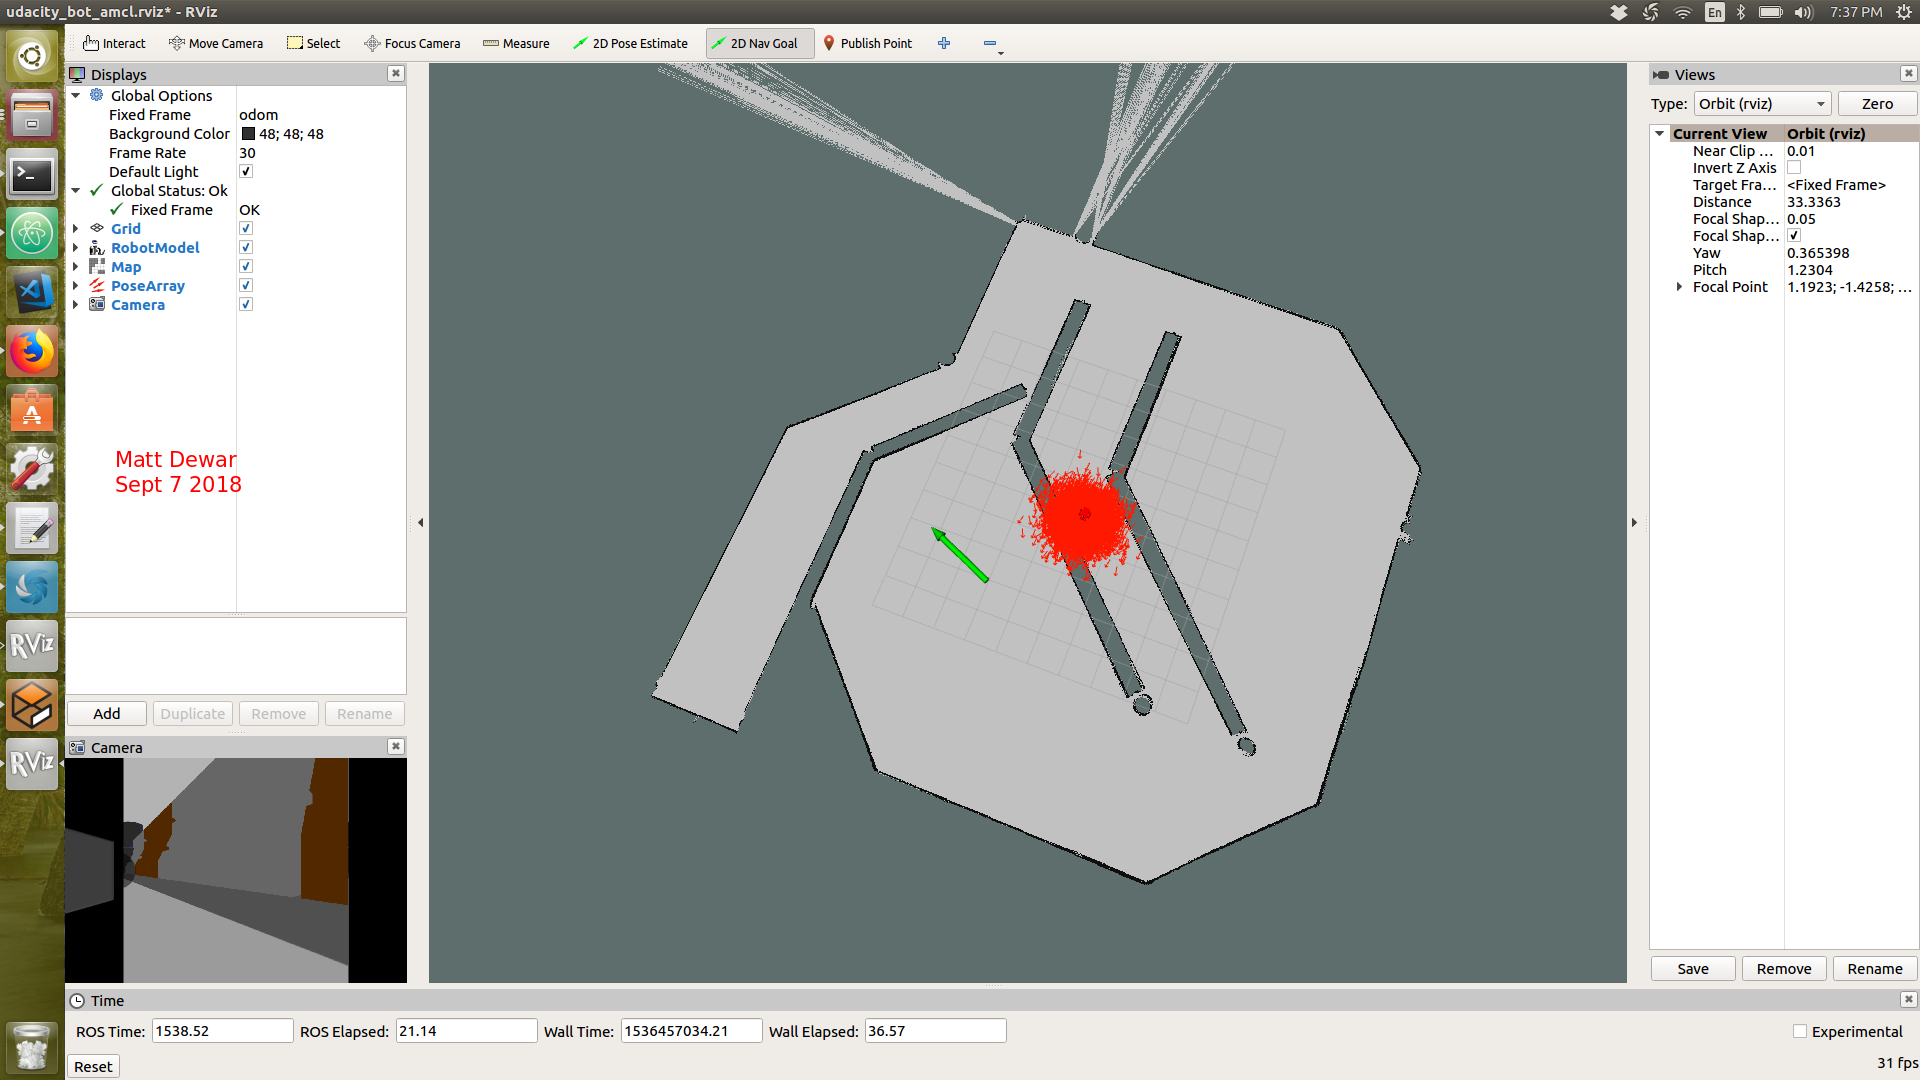
\includegraphics[width=\linewidth]{../img/rviz_2DNavGoal.png}
    \caption{Running 2D Nav Goal in RViz}
    \label{fig:2DNavGoal}
\end{figure}

Without local planner parameters the robot had hard time navigating down the hallway, zigzagging back and forth down the hall, getting stuck against walls and having to reverse out of them. During testing the local planner was throwing collision errors when the robot was getting too close to walls, however eventually made it to its destination.

Adding AMCL filter parameters, laser model parameters, and odometery model parameters provided drastic increases to the performance of the localization node, and the local planner node. Decreasing the amount of particles available for monte carlo localization aided in performance, and helped decrease uncertainty, however also decreased the accuracy of the localization. The KLD sampling were shown to be tuned appropriately where after a certain amount of time sets number of mone carlo particles was minimized, and were seen to be tightly centered around the robots actual pose. Figure. \ref{fig:afterAMCLParam} Shows the improvement after adding the AMCL parameters.

\begin{figure}[thpb]
    \centering
    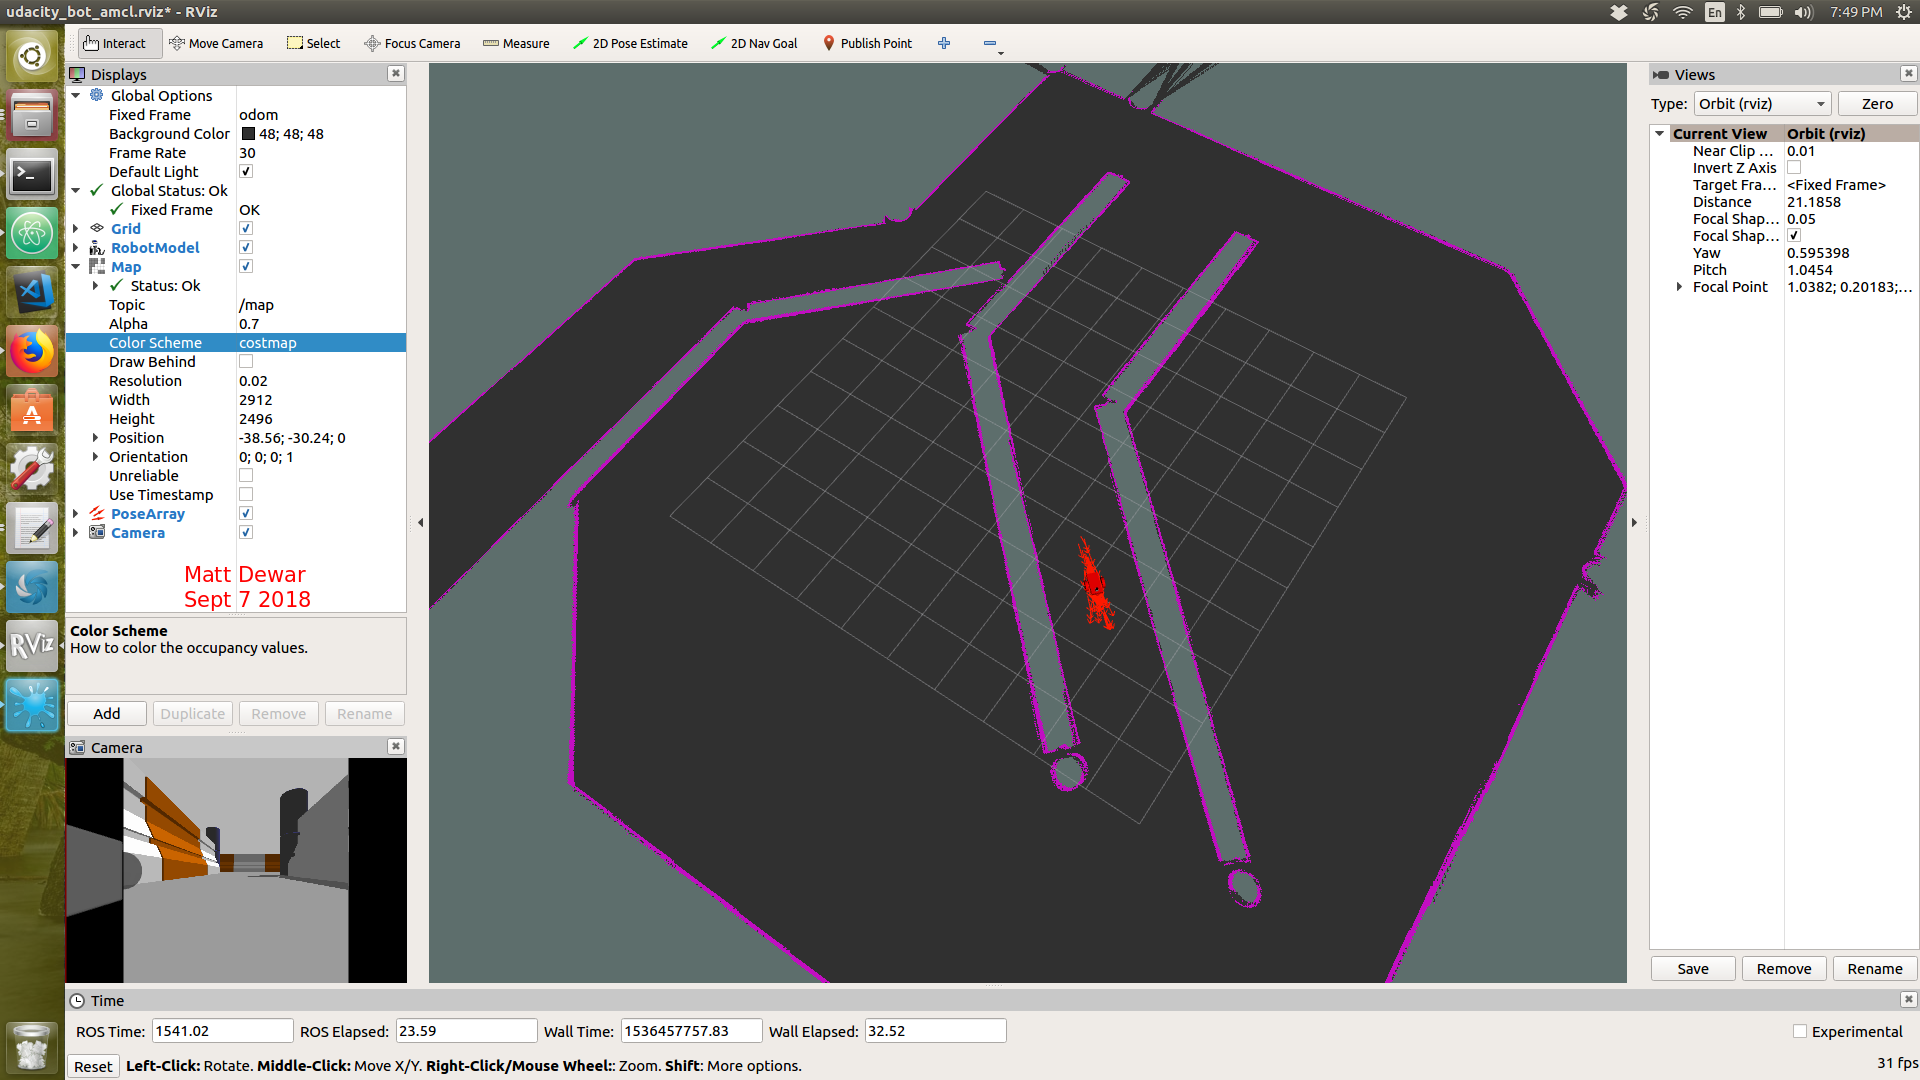
\includegraphics[width=\linewidth]{../img/rviz-w-amcl-param.png}
    \caption{Localization of benchmark robot after adding AMCL node parameters.}
    \label{fig:afterAMCLParam}
\end{figure}

Upon running the \textit{$navigation goal.cpp/$} unit test on the optimization configuration parameters the robot was seen to navigate quickly and effectively through the narrow corridor, and was able to turn around the bottom corner obstacle in one smooth motion. However once it reached the proper position the robot had difficulty assuming the correct orientation of the goal pose, rotating around a few times before completing the script. Figure. \ref{fig:benchmarkNavGoal} shows the benchmark robot reaching the navigation goal within 1 minute and 47 seconds.

\begin{figure}[thpb]
    \centering
    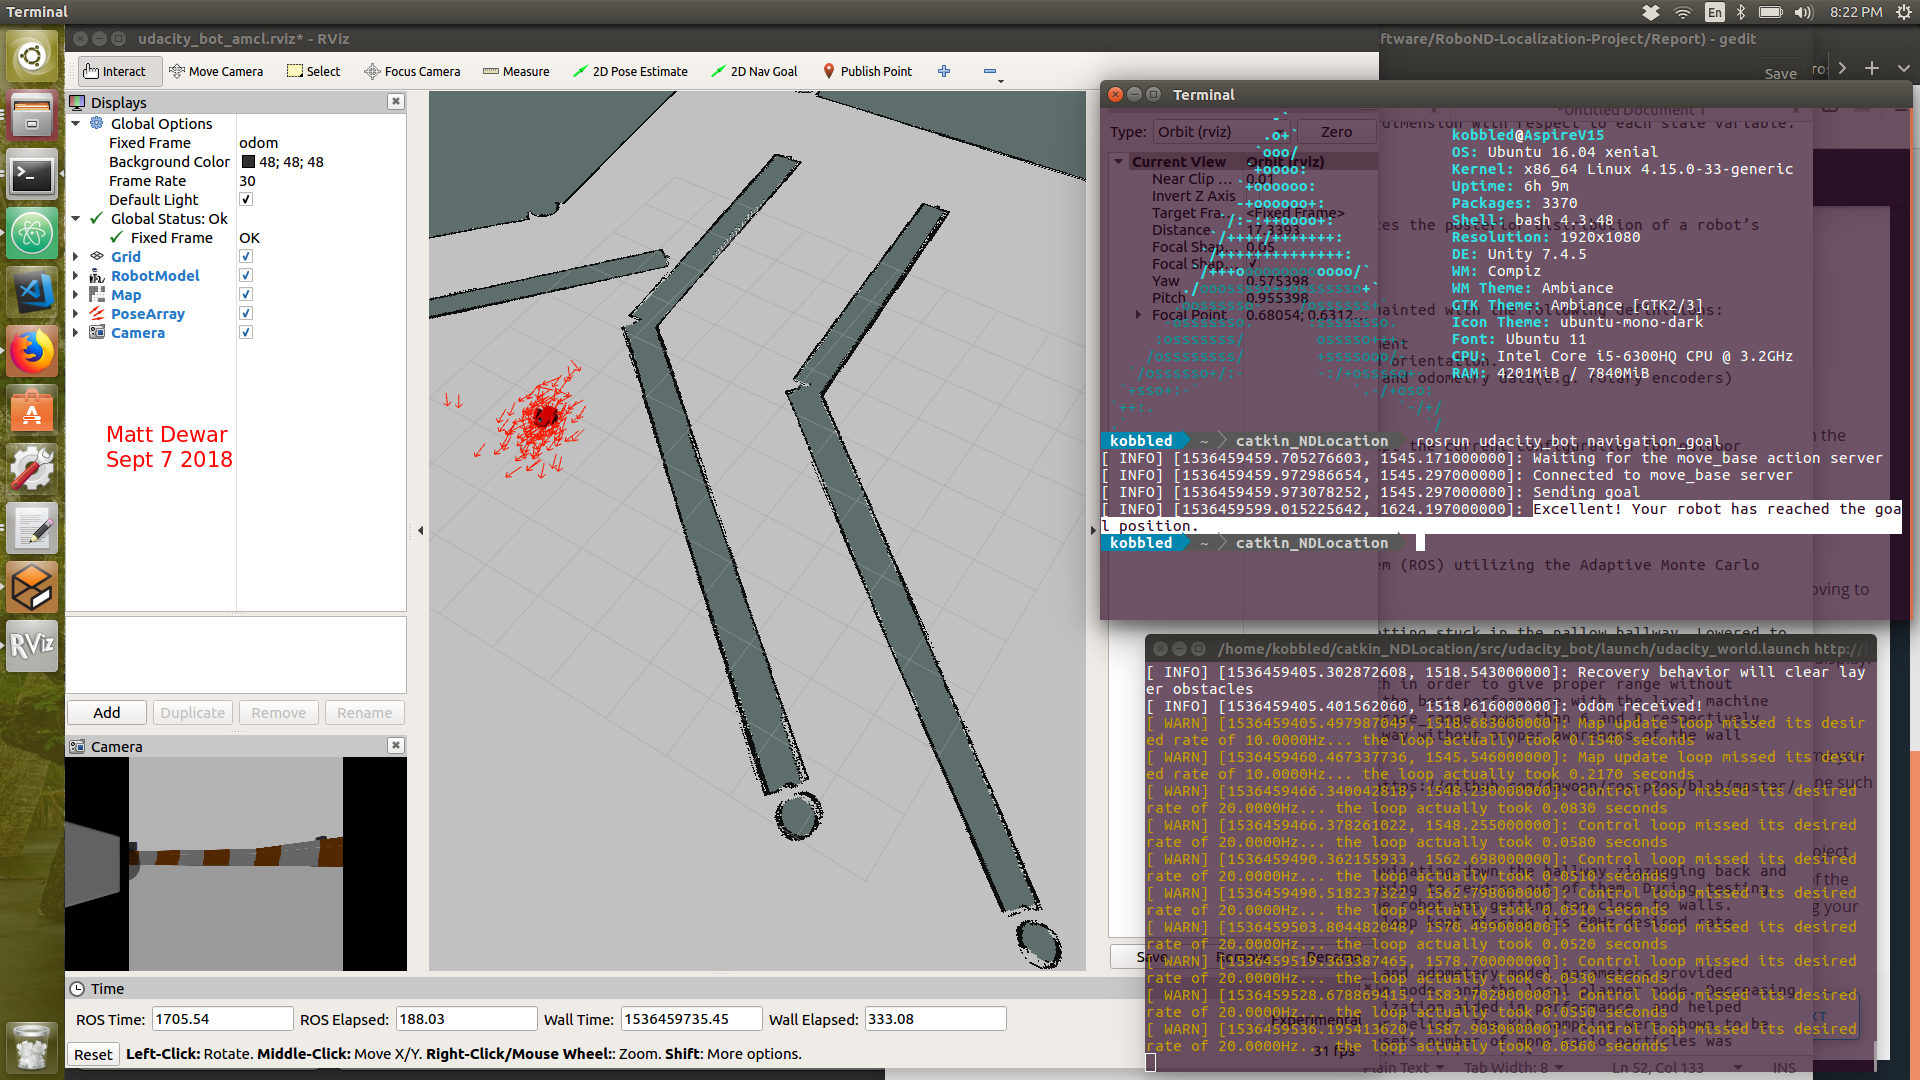
\includegraphics[width=\linewidth]{../img/reached_navigation_goal.png}
    \caption{Benchmark robot reaching the navigation objective set for this project.}
    \label{fig:benchmarkNavGoal}
\end{figure}



\subsubsection{Student}\label{sec:student}

The Tank-bot had a much more difficult time navigating than the benchmark bot, where numerous iteration on configuration parameters were experimented with, however none yielded successful results. Figure. \ref{fig:tankbotissues} illustrates some problems with the Tank-bot, particularly with the orientation that the robot starts in, attempting a three point turn within the corridor in order to reorient itself. This namely results in the Tank-bot eventually erroring out, and not completing the navigation goal. Teleop was used to try an identify if there were any intrinsic locomotion problems with the model. While an issues with the robot wheels at different heights causing instability was addressed, handling multiple wheels with the differential drive controller was unable to be solved for this report. Responsiveness of the robot appeared to be hindered by the extra wheel on the side either not stopping on rotation, or not moving appropriately with the given teleop command. Differential drive on all three wheels was investigated with the best response coming from a rear wheel drive configuration. Attempts were made to chain the wheels together in a controller configuration YAML file, however integrating that with the other topics and packages in this software proved challenging and were unsolved at the time of writing this.


\begin{figure}[thpb]
    \centering
    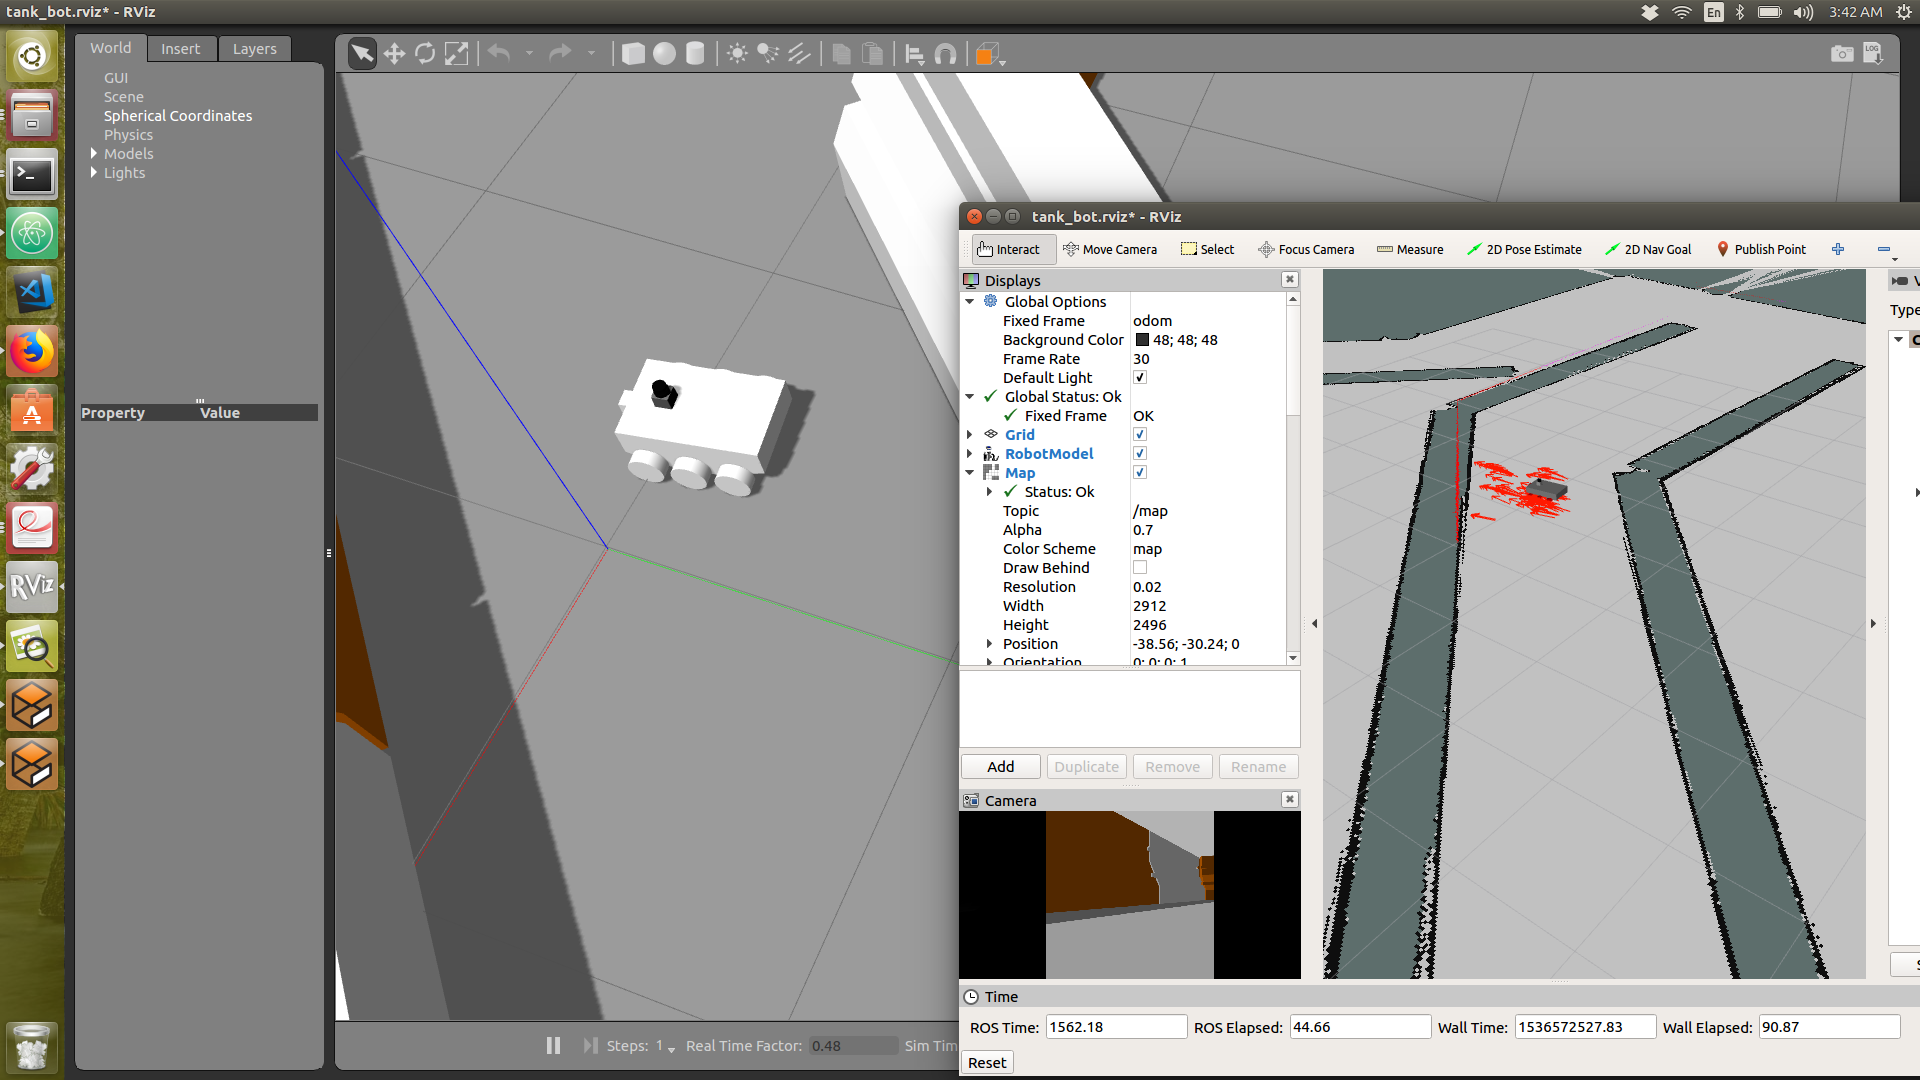
\includegraphics[width=\linewidth]{../img/tank-bot-issues2.png}
    \caption{Issues with the Tank-bot resulted in a solution for the Tank-bot to not be found.}
    \label{fig:tankbotissues}
\end{figure}

\section{Discussion}

With great success of parameter optimization on the benchmark robot, the assumption that the navigation stack could be easily ported over to other robot platform proved false. The personal robot model was almost completely unresponsive to the parameters of the benchmark model that were able to solve the navigation goal test. At the time of writing this report the personal robot was unable to reach the goal destination. As mentioned in section \ref{sec:student}, problems with the differential controller on a multi wheel robot were discovered and unsolved. If the diff\_drive\_controller package can be configured in such a way as to provide control of all the wheels, or if independent control of multiple wheels with a skid steer controller can be used, the navigation problems of the Tank-bot may be able to be distilled down to a locomotion issue.

Turning around in the narrow corridor seems to be the edge case for the navigation stack presented in this project. While turning in the corridor is the Achilles heal for the Tank-bot, the benchmark robot was observed to struggle in the same case, but eventually be able to recover out of it. Parameter testing shows that the inflation radius, obstacle range, and robot radius all need to be minimized in order to be able to rotate within a tight corridor. However after dozens of tests on the Tank-bot appropriate parameters could not be found.

In the kidnapped robot problem the robot is removed the environment, and randomly placed at a new location within the environment. From observations made in this project it can be stated that the AMCL would work well in solving the kidnapped robot problem as it is not completely dependant on the initial position of the robot, and after a few time steps should be able to start localizing.

In an outdoor environment AMCL would be useful in locating objects within a mapped terrain. For example locating boreholes for geological surveying operations is a tedious task that could be automated by way of surveying robots. Moreover, finding missing persons or equipment in a forest or other sheltered terrain could be done with a robot equipt with AMCL.

\begin{comment}
This is the only section of the report where you may include your opinion. However, make sure your opinion is based on facts. If your robot performed poorly, make mention of what may be the underlying issues. If the robot runs well, which aspects contribute to that? Again, avoid writing in the first person (i.e. Do not use words like "I" or "me"). If you really find yourself struggling to avoid the word "I" or "me"; sometimes, this can be avoid with the use of the word “one”. As an example: instead of : "I think the robot cannot localize itself because the sensor does not provide enough information for localization" try: "one may believe the localization performance is poor because the sensor layout is not able to provide enough information for localization". They say the same thing, but the second avoids the first person.

- Which robot performed better?
- Why it performed better? (opinion)
- How would you approach the 'Kidnapped Robot' problem?
- What types of scenario could localization be performed?
- Where would you use MCL/AMCL in an industry domain?
\end{comment}


\section{Conclusion / Future work}

In conclusion a navigation stack with AMCL localization was successfully implemented on the benchmark robot provided for this project, completing the navigation goal unit test in 1 minute and 47 seconds. A personal robot was developed that was drastically different than the benchmark robot, however the increased complexity of the wheel design proved to be outside of the scope of this project. Tuning of costmap and AMCL parameters greatly increase the ability, and efficiency of the navigation and localization of the robots, however a solution was unable to be found for the personal robot.

Moving to a machine with higher computational resources, particle sizes should be increased to improve accuracy of the localization.

For the personal robot a restructured differential drive controller or skid steer controller should be developed. Once the robot is able to navigate and localize, redesigning the sensors in order to adapt to outdoor environments will be crucial. It is recommended to try modelling two laser scanner at different height (one on the bottom, and one on top), to be able to identify obstacles into categories that the robot can, and cannot traverse. From here an outdoor simulated environment can be tested to evaluate the proficiency of this model for such a case.

\begin{comment}
This section is intended to summarize your report. Your summary should include a recap of the results, did this project achieve what you attempted, how would you deploy it on hardware and how could this project be applied to commercial products?
For Future Work, address areas of work that you may not have addressed in your report as possible next steps. This could be due to time constraints, lack of currently developed methods / technology, and areas of application outside of your current implementation. Again, avoid the use of the first-person.
\end{comment}



\bibliography{bib}
\bibliographystyle{ieeetr}

\end{document}
